
\section{Python Code}
\subsection{Binarisation and Filtering}
\subsubsection{Binary Mask}
\begin{minted}{python}
mask = im > 0.8 # bright pixels will be True in the mask, others will be False
plt.imshow(mask)
\end{minted}
\begin{center}
	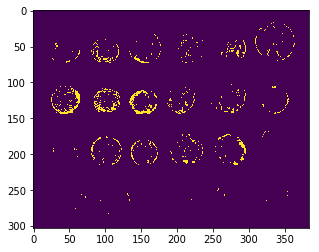
\includegraphics[width=0.4\linewidth]{img/BinaryMask.png}
\end{center}

\subsubsection{Connected Component Analysis}
\begin{minted}{python}
import skimage.measure
labels = skimage.measure.label(im > 0.5)
print(labels.shape, labels.dtype)
print("Unique values in labels:", np.unique(labels))
> (303, 384) int64
> Unique values in labels: [  0   1   2   3   4   5   6   7   8   9  10
> 11  12  13  14  15  16  17  18  19  20  21  22  23  24  25  26  27  28
> 29  30  31  32  33  34  35  36  37  38  39  40  41  42  43  44  45  46
> 47  48  49  50  51  52  53  54  55  56  57  58  59  60  61  62  63  64
> 65  66  67  68  69  70  71  72  73  74  75  76  77  78  79  80  81  82
> 83  84  85  86  87  88  89  90  91  92  93  94  95  96  97  98  99 100
> 101 102 103 104 105 106 107  108 109 110 111 112 113 114 115 116 117 118 119]

regions = skimage.measure.regionprops(labels)

large_regions = [r for r in regions if r.area > 100]

# equivalent to
large_regions = []
for r in regions:
	if r.area > 100:
		large_regions.append(r)

print(f"There are {len(large_regions)} large regions")
> There are 25 large regions
\end{minted}
\noindent
The \mintinline{python}{regionprops} (documentation) function can compute properties for each connected component. Some important properties are the following:
\begin{itemize}[label=,nosep,leftmargin=*, labelindent=0.5cm]
	\item \mintinline{python}{area : int} Number of pixels of the region.
	\item \mintinline{python}{bbox : tuple} Bounding box (\texttt{min\_row, min\_col, max\_row, max\_col}).
		Pixels belonging to the bounding box are in the half-open interval \texttt{[min\_row; max\_row)} and [min\_col; max\_col).
	\item \mintinline{python}{centroid : array} Centroid coordinate tuple (row, col).
	\item \mintinline{python}{convex_area : int} Number of pixels of convex hull image, which is the smallest convex polygon that encloses the region.
	\item \mintinline{python}{label : int} The label in the labeled input image.
\end{itemize}

\begin{minted}{python}
import matplotlib.patches as patches
fig, ax = plt.subplots()
ax.imshow(im, cmap="gray")
for r in large_regions:
	(min_row, min_col, max_row, max_col) = r.bbox
	width = max_col - min_col
	height = max_row - min_row
	rect = patches.Rectangle((min_col,min_row),width,height,
	linewidth=1,edgecolor='b',facecolor='none')
	ax.add_patch(rect)
\end{minted}

\begin{minted}{python}
background = (np.min(im,axis=1,keepdims=True) * np.ones((1,im.shape[1])))

fig, axs = plt.subplots(ncols=2, nrows=2, figsize = (13,13))
axs[0,0].imshow(im, vmin=0, vmax=1)
axs[0,0].set(title="original")
axs[0,1].imshow(background, vmin=0, vmax=1)
axs[0,1].set(title="background")
axs[1,0].imshow(im - background, vmin=0, vmax=1)
axs[1,0].set(title="im - background")
mask = (im - background) > 0.25
axs[1,1].imshow(mask, vmin=0, vmax=1)
axs[1,1].set(title="binarized")
\end{minted}
\begin{center}
	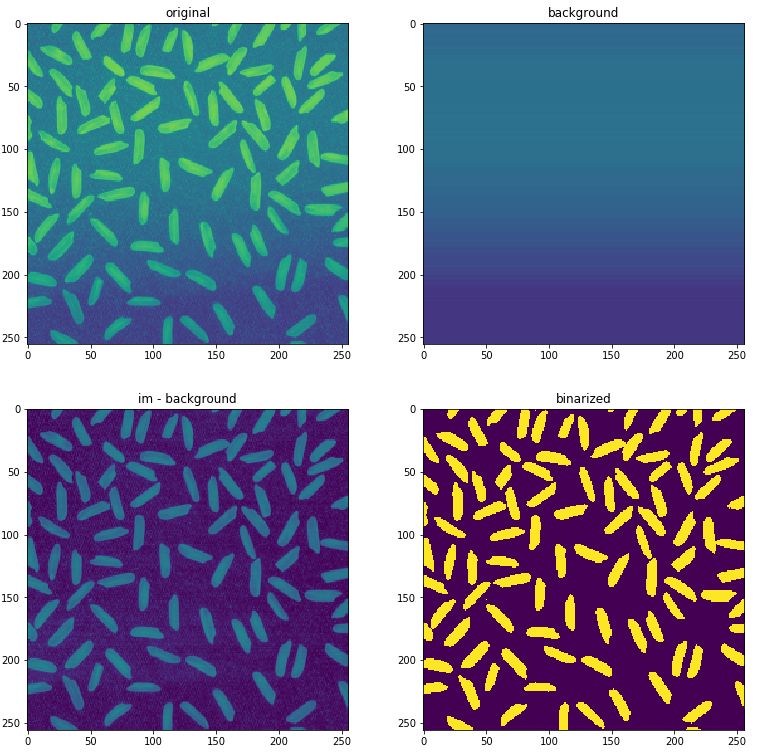
\includegraphics[width=0.7\linewidth]{img/BinarizedRiceGrains}
\end{center}

\subsection{Model Fitting Hough Lines}
\begin{minted}{python}
import skimage.feature
import skimage.transform.hough_transform as ht
import matplotlib.pyplot as plt
import numpy as np

import skimage.data
import skimage.feature

im = skimage.data.camera()
imedges = skimage.feature.canny(im)

lines = ht.probabilistic_hough_line(imedges, threshold=100)
len(lines)

# Draw detected lines
fig,ax = plt.subplots(figsize=(10,10))

ax.imshow(im,cmap="gray")
for ((x0,y0),(x1,y1)) in lines:
ax.plot([x0,x1],[y0,y1],'b-')
\end{minted}

\subsection{Superpixel Segmentation}
\begin{minted}{python}
# import the necessary packages
from skimage.segmentation import slic
from skimage.segmentation import mark_boundaries
from skimage.util import img_as_float
from skimage import io
import matplotlib.pyplot as plt
import argparse

# construct the argument parser and parse the arguments
ap = argparse.ArgumentParser()
ap.add_argument("-i", "--image", required = True, help = "Path to the image")
args = vars(ap.parse_args())

# load the image and convert it to a floating point data type
image = img_as_float(io.imread(args["image"]))

# loop over the number of segments
for numSegments in (100, 200, 300):

# apply SLIC and extract (approximately) the supplied number
# of segments
segments = slic(image, n_segments = numSegments, sigma = 5)

# show the output of SLIC
fig = plt.figure("Superpixels -- %d segments" % (numSegments))
ax = fig.add_subplot(1, 1, 1)
ax.imshow(mark_boundaries(image, segments))
plt.axis("off")

# show the plots
plt.show()
\end{minted}
